\newpage
\section{Frequenzweichen}

\subsection*{Tiefton- und Hochton-Weiche}\label{sec:4.3}
\subsubsection{Allgemeines}\label{subsec:4.3.1}
Für die Satellitenlautsprecher, welche aus einem Hochton-Lautsprecher und einem Tiefton-Lautsprecher bestehen werden nun die Teilfrequenzbereiche Mitte und Hoch benötigt.
Da es sich bei dem Satellitenboxen um ein Paar an Boxen handelt und diese räumlichen weiter entfernt voneinander stehen, können nun Stereo-Effekte verwendet und mit dem reinen Stereo-Audio-Eingangssignal gearbeitet werden.
Eine Aufteilung des Signals in Linke- und Rechte-Satellitenbox muss jedoch schon getroffen werden, um die Effekte richtig zu erhalten.
Dafür wird für die Linke- und Rechte-Satellitenbox, jeweils bestehend aus Hochton- und Tiefton-Lautsprecher, die entsprechende Weichen verwendet.\\
Das Audiosignal soll so gefiltert werden, dass der Hochton-Lautsprecher nur Frequenzen über 1,5kHz und der Tiefton-Lautsprecher Frequenzen bis 6kHz zum Abstrahlen erhält.
Obwohl es den Mono-Subwoofer gibt der die untersten Frequenzen (<150Hz) abzustrahlen hat, dürfen die Satelliten-Tiefton-Lautsprecher im selbigen Bereich ebenfalls spielen.
Somit wird die abstrahlende Fläche vergrößert und freiwerdende absolute Pegel höher.
Bei dem Satelliten-Tiefton-Lautsprecher wird jedoch ein Bandpass vorgesehen um bei möglichen Resonanzen mit dem Mono-Subwoofer das Audiosignal filtern zu können.\\
Dementsprechend sollen die Weichen gewählt und designet werden.\\

\subsubsection{Schaltung}\label{subsec:4.3.2}
Das Eingangssignal (Links, Rechts, Masse) wird an einer dreipoligen Stiftleiste angeschlossen (Abb. \ref{fig:4.3.2.1}).
Zuerst gelangt Signal-Links und -Rechts an jeweils ein Potentiometer um den Pegel anpassen zu können, es bietet also eine Regelmöglichkeit.
Über das Widerstandsnetzwerk am Plus-Eingang von HTA, welcher mit jedem Plus-Eingang der anderen OPVs verbunden ist, wird der Arbeitspunkt eingestellt (Siehe Kapitel \ref{subsec:3.5.1}). 
%TD Arbeitspunkt Verweis
Es folgen die Weichen.
Hochpass-Weiche für Links/Rechts und Tiefpass-Weiche für Links/Rechts.
Ein \enquote{Butterworth-Tiefpass-Weiche 2. Ordnung} wurde bereits in dem Kapitel \ref{subsec:4.1.3} erklärt.
Das \enquote{Butterworth-Hochpass-Weiche und -Bandpass-Weiche 2. Ordnung} weist keine groben Unterschiede auf, der Unterschied liegt lediglich in der Bauteilaufteilung.\\
Nach der Weiche gelangen die frequenzmäßig getrennten Signale zu deren Ausgangspunkt. Es ist für jede Signalleitung eine zweipolige Stiftleiste vorgesehen (Signal \& Masse), da der darauffolgende Verstärker selbige Verbindung als Eingang vorweist.
Die Stiftleisten sind jedoch gruppiert nach Bandpass- und Hochpass-Ausgang.\\
\begin{figure} [H]
	\centering	
	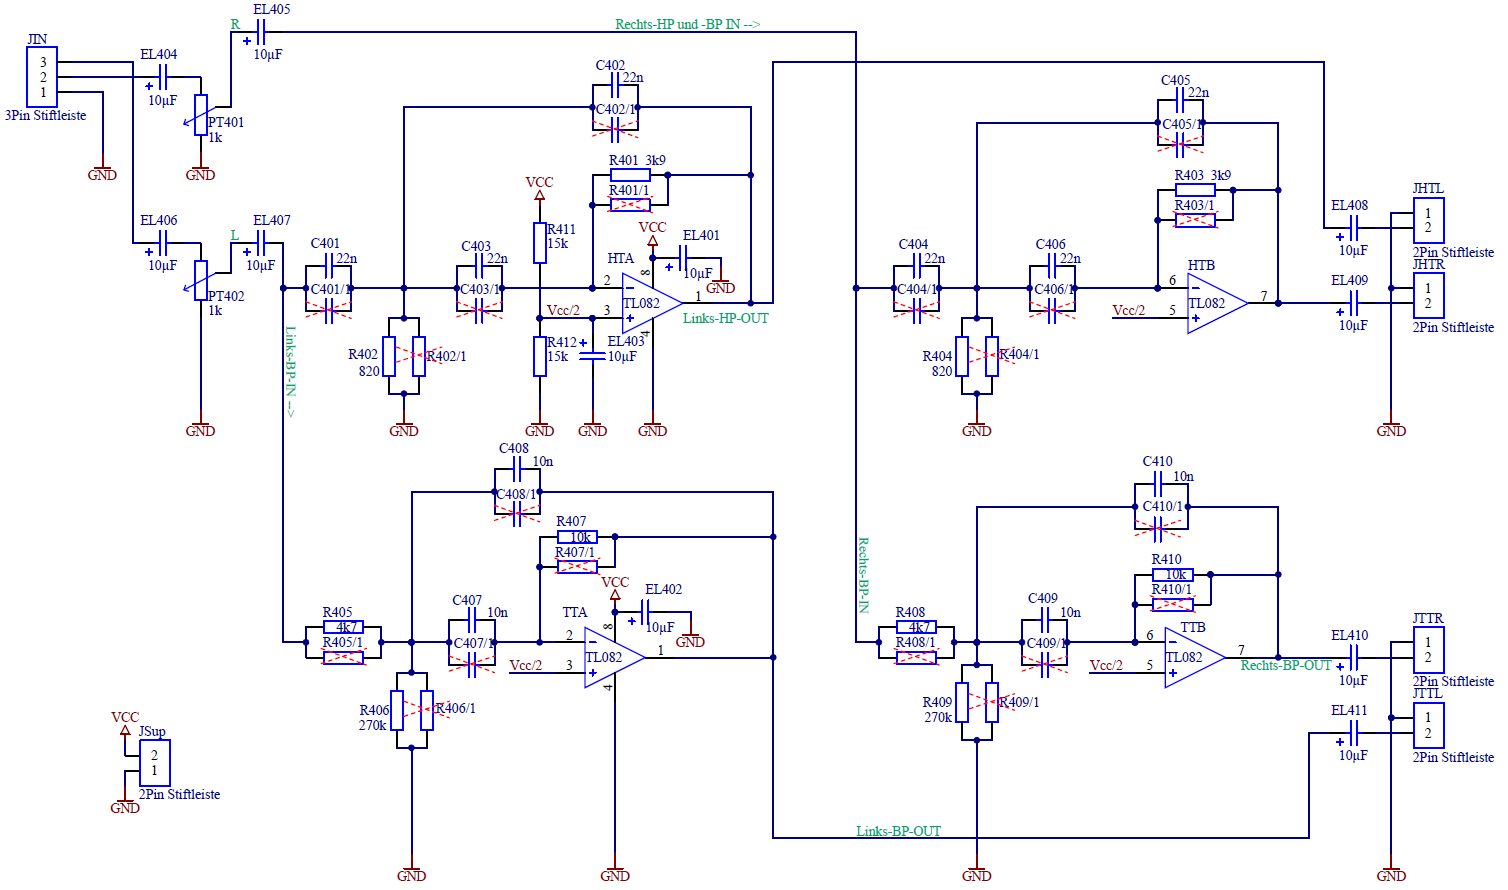
\includegraphics[width=1\textwidth]{img/Print4/4_TTuHTWeiche-Schematic.PNG}
	\caption{Butterworth-Bandpass-Weiche 2. Ordnung}
	\label {fig:4.3.2.1}
\end{figure}
%TD Layout anpassen --> Abstand zu groß!
Eine der Bandpass-Weiche.
Gut sichtbar die doppelte, parallele Ausführung von Widerständen und Kondensatoren um krumme Werte auch erhalten zu können.
Bedingt durch Parallel-Schaltung von Widerständen und Kondensatoren.\\ 
Der Eingang wurde gespiegelt um ein schöneres Bild zu erlangen.
Die Spiegelung ist für das PCB-Layout nicht relevant!\\
Bedingt durch die Versorgungsspannung ist auch der Spannungsteiler für $\frac{Vcc}{2}$ am Plus-Eingang des OPVs implementiert.
\begin{figure} [H]
	\centering	
	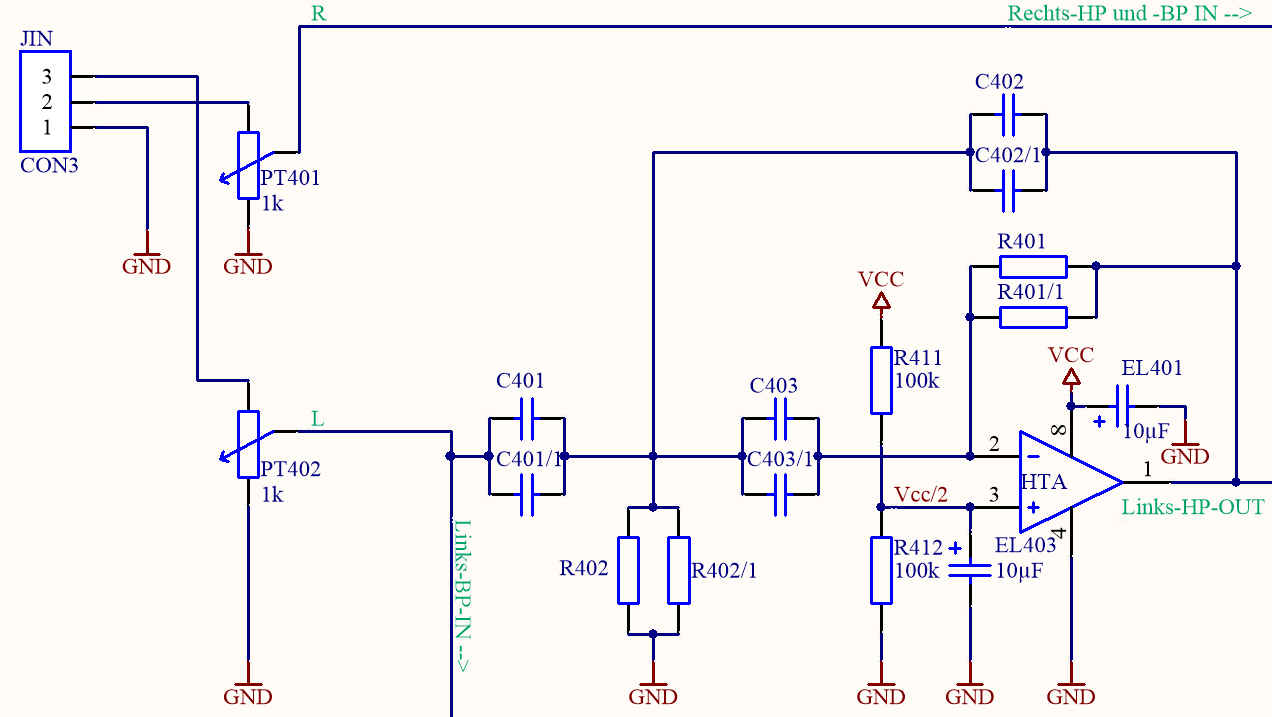
\includegraphics[width=0.9\textwidth]{img/Print4/4_TTuHTWeiche-LinksHP-Schematic.PNG}
	\caption{Butterworth-Bandpass-Weiche 2. Ordnung - aus Abb.\ref{fig:4.3.2.1}}
	\label {fig:4.3.2.2}
\end{figure}
Am B-Teil des OPVs (erkennbar an der Beschriftung: TT\enquote{B}) ist keine Versorgung einzuzeichnen, da er mit dem A-Teil einen achtpinnigen IC mit zwei integrierten OPVs ergibt.
Die zwei Teile sind über das IC-Gehäuse mit der gleichen Versorgungsspannung verbunden, deshalb ist das einmalige Kennzeichnen ausreichend.\\
\begin{figure} [H]
	\centering	
	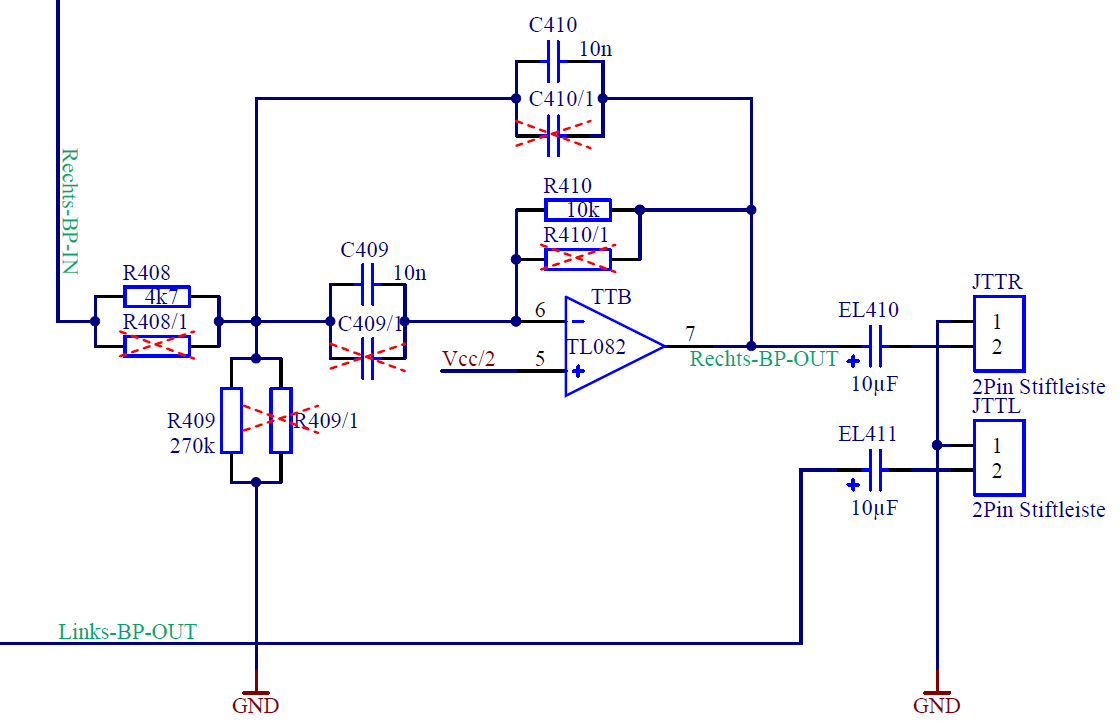
\includegraphics[width=0.7\textwidth]{img/Print4/4_TTuHTWeiche-RechtsBP-Schematic.PNG}
	\caption{Butterworth-Bandpass-Weiche 2. Ordnung - aus Abb.\ref{fig:4.3.2.1}}
	\label {fig:4.3.2.3}
\end{figure}

\newpage
\subsubsection{PCB}\label{subsec:4.3.3}
Es werden die grundlegenden Regeln zur Leiterplattenentflechtung angewandt (\ref{subsec:3.1.2}).
%TD Leiterplattenentflechtung Regeln Verweis
Bei dem Design (Abb. \ref{fig:4.3.3.1}) wird auf hohe Variierbarkeit geachtet um auch zB. Kondensatoren mit unterschiedlichen Fußabdruck (engl. \enquote{Footprint}) verwenden zu können.\\
Es wurden ebenfalls nahe an den OPVs ELKOs \enquote{EL401, EL402} zwischen Versorgungsspannung und Masse verbaut, um Störungen zu verhindern.
\begin{figure} [H]
	\centering	
	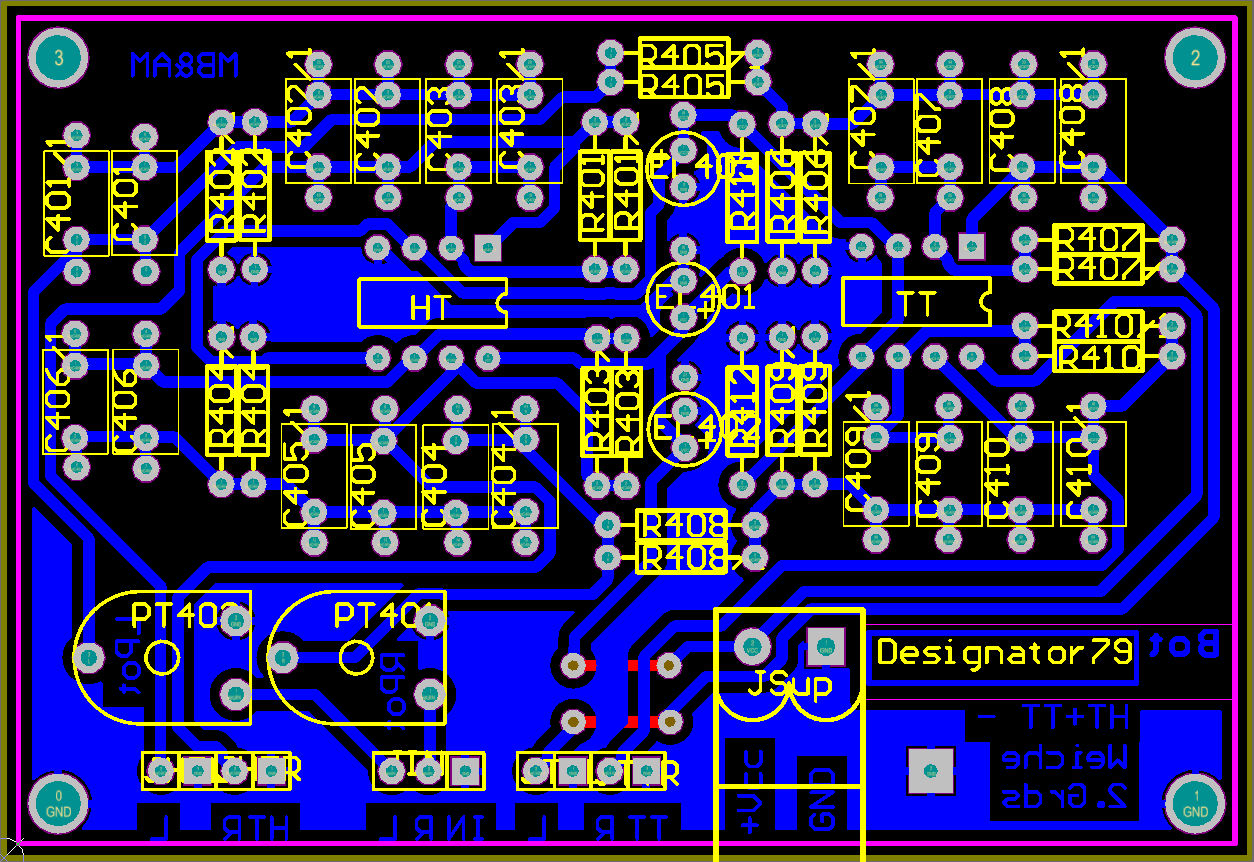
\includegraphics[width=1\textwidth]{img/Print4/4_TTuHTWeiche-PCB.PNG}
	\caption{Tiefton- und Hochtonweichen - PCB}
	\label {fig:4.3.3.1}
\end{figure}

%---------------------------------------------------------------------------------%

\newpage
\subsection*{Mono-Subwoofer-Addier-Schaltung und Mono-Subwoofer-Weiche}\label{sec:4.2}
\subsubsection{Allgemeines}\label{susec:4.2.1}
Das empfangene Audio-Signal muss für das Lautsprecher-System aufgetrennt werden. In Hoch-, Mitte- und Tiefton-Bereich.
Für den \enquote{Mono-Subwoofer} werden nur die tiefen Frequenzen des Audiosignals verwendet.
Da, wie der Name schon sagt, es sich um einen \enquote{Mono-Subwoofer} handelt, muss das Stereo-Audio-Signal zuvor mittels OPV-Addierschaltung addiert werden um ein Mono-Audio-Signal zu erhalten.\\
Es soll eine Platine angefertigt werden, welcher über eine OPV-Addierschaltung verfügt und des weiteren das eintreffende Audio-Signal über ein Weiche passend für den \enquote{Mono-Subwoofer} filtert.
Diese Schaltung für die Tiefpass-Weiche muss variabel designet werden. Die Tiefpass-Weiche muss unabhängig vom Platinendesign, nur durch Ändern von Bauteilwerten, andere Grenzfrequenzen umsetzen können.

\subsubsection{Schaltung}\label{subsec:4.2.2}
Passend dem Signalverlauf sitzt am Beginn der Schaltung (Abb. \ref{fig:4.2.2.1}) die erste Regelung über zwei Potentiometer.
Anschließend kommt man zu der Addier-Schaltung welche das Stereo-Audiosignal in ein Mono-Audiosignal wandelt und dadurch Stereo-Effekte wie zB. Balance am \enquote{Mono-Subwoofer} entfernt.\\
Bedingt durch die asymmetrische Spannungsversorgung muss am Plus-Eingang des OPV ein Arbeitspunkt eingestellt werden (Siehe Kapitel \ref{subsec:3.5.1}).\\
%TD Arbeitspunkt Verweis
Um Störungen im OPV zu vermeiden wird sehr nahe an diesem der ELKO \enquote{EL301} zwischen Versorgungsspannung und Masse vorgesehen.\\
Nach Addieren des Stereo-Audiosignals zu einem Mono-Audiosignal kommt dieses zur Aktiven-Tiefpass-Weiche.
Bevor das gefilterte Signal weiter zum Verstärker läuft wird nochmals die Möglichkeit geboten um die Amplitude des Signals anzupassen.
\begin{landscape}
	\vspace*{\fill}
	\begin{figure} [H]
		\centering
		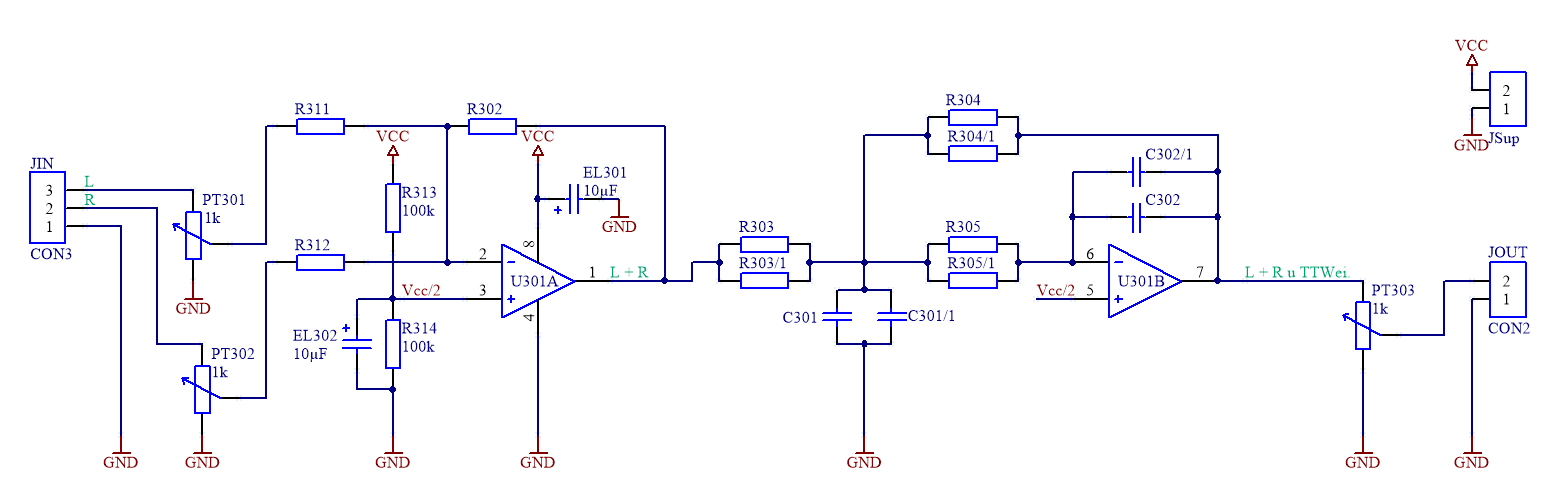
\includegraphics[width=\linewidth,height=0.9\textheight,keepaspectratio]{img/Print3/3mTTWeicheruAddiererDiplSchematic.PNG}
		\caption{Schematic Mono-Subwoofer-Addier-Schaltung und Mono-Subwoofer-Weiche}
		\label {fig:4.2.2.1}
	\end{figure}
	\vfill
\end{landscape}
\raggedbottom


\subsubsection{PCB}\label{subsec:4.2.3}
An einer der vier Seiten der Leiterplatte (Abb. \ref{fig:4.2.3.1})(in diesem Fall: Unten) wurden alle wesentlichen Ein- und Ausgänge platziert.
Eine dreipolige Eingangsstiftleiste für Rechts, Links und Masse.
Eine zweipolige Ausgangsstiftleiste für Signal und Masse.
Es dürfen bei Ein- und Ausgang noch Stiftleisten verwendet werden, da es sich hier noch um geringe Spannungen und Ströme handelt.\\
Des weiteren darf die Spannungsversorgung nicht fehlen.
Wegen größeren Spannungen wurden massivere Stecker verwendet.
In diesem Fall handelt es sich um steckbare Pol-Klemmen.
Zum Testen wurde ein zusätzlicher Masse-Printstift angebracht um bei Messungen mit einem Oszilloskop einen besseren Massebezugspunkt zu haben.\\
Die Bauteile wurden nach Möglichkeit gestaffelt, beziehungsweise gruppiert auf der Leiterplatte platziert um den Platzbedarf zu minimieren.\\
Es wurde grundsätzlich auf jeder Platine versucht eine geeignete Beschriftung vor zu sehen um Außenstehenden die Handhabung mit der Platine ebenfalls zu ermöglichen. Masse wurde selten beschriftet, da eine Massefläche verwendet wurde und daher die Masseverbindungen sehr gut ersichtlich sind.
\begin{figure} [H]
	\centering
	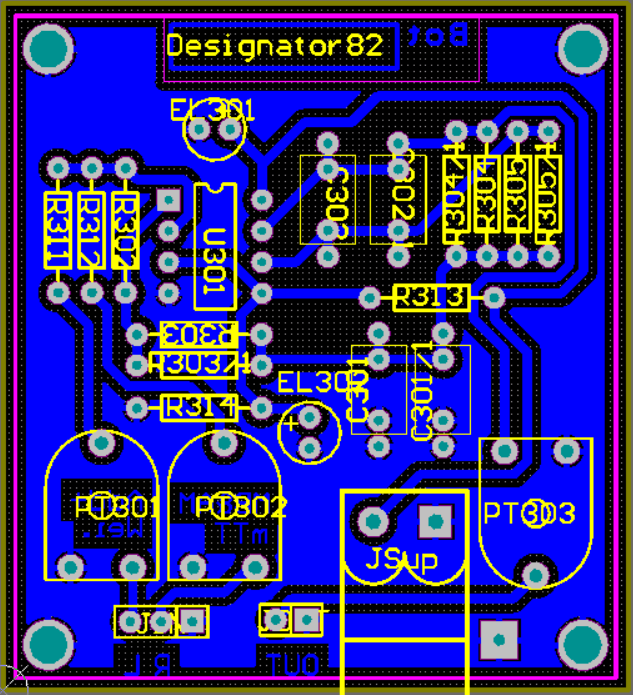
\includegraphics[width=0.7\textwidth]{img/Print3/3mTTWeicheruAddierer-PCB.PNG}
	\caption{PCB}
	\label {fig:4.2.3.1}
\end{figure}














